\graphicspath{{./1-Proyecto/capitulo1/}}

\chapter{ADM}

\section{Introducción}
TOGAF (The Open Group Architecture Framework) es un marco de referencia ampliamente reconocido para el desarrollo de Arquitectura Empresarial (AE). Este estándar proporciona un enfoque estructurado, detallado y formal, complementado con un conjunto de herramientas que permiten definir, implementar y evolucionar una arquitectura organizacional efectiva. La AE cumple dos propósitos fundamentales: primero, guiar la implementación de sistemas mediante una descripción precisa y coherente; y segundo, ofrecer una representación estructurada de los componentes de la organización, sus relaciones, directrices de gobierno y evolución en el tiempo. \cite{why_is_important_ADM}

En este contexto, TOGAF facilita la estandarización de arquitecturas al considerar todos los procesos organizacionales. Para expresar correctamente estas necesidades, se requiere un lenguaje común que permita establecer una visión integral de la AE. Archimate, lenguaje soportado por The Open Group, cumple esta función. Su utilidad radica en describir, analizar y visualizar los diferentes dominios de la empresa y sus interrelaciones, proporcionando una comprensión clara de la arquitectura del negocio. \cite{definicion_puntos_de_vista}

Este capítulo presenta los conceptos fundamentales del Método de Desarrollo de Arquitectura (ADM), así como una introducción a Archimate y sus componentes clave.

\section{¿Qué es ADM?}
El \textbf{Architecture Development Method} (ADM) es el núcleo metodológico de TOGAF. Se trata de un marco estructurado para planear, desarrollar, implementar y gestionar la arquitectura empresarial de forma iterativa y controlada. Su propósito es asegurar que la arquitectura se alinee constantemente con las necesidades estratégicas y operativas de la organización. \cite{ADM_definition}

\begin{figure}[H]
	\centering
	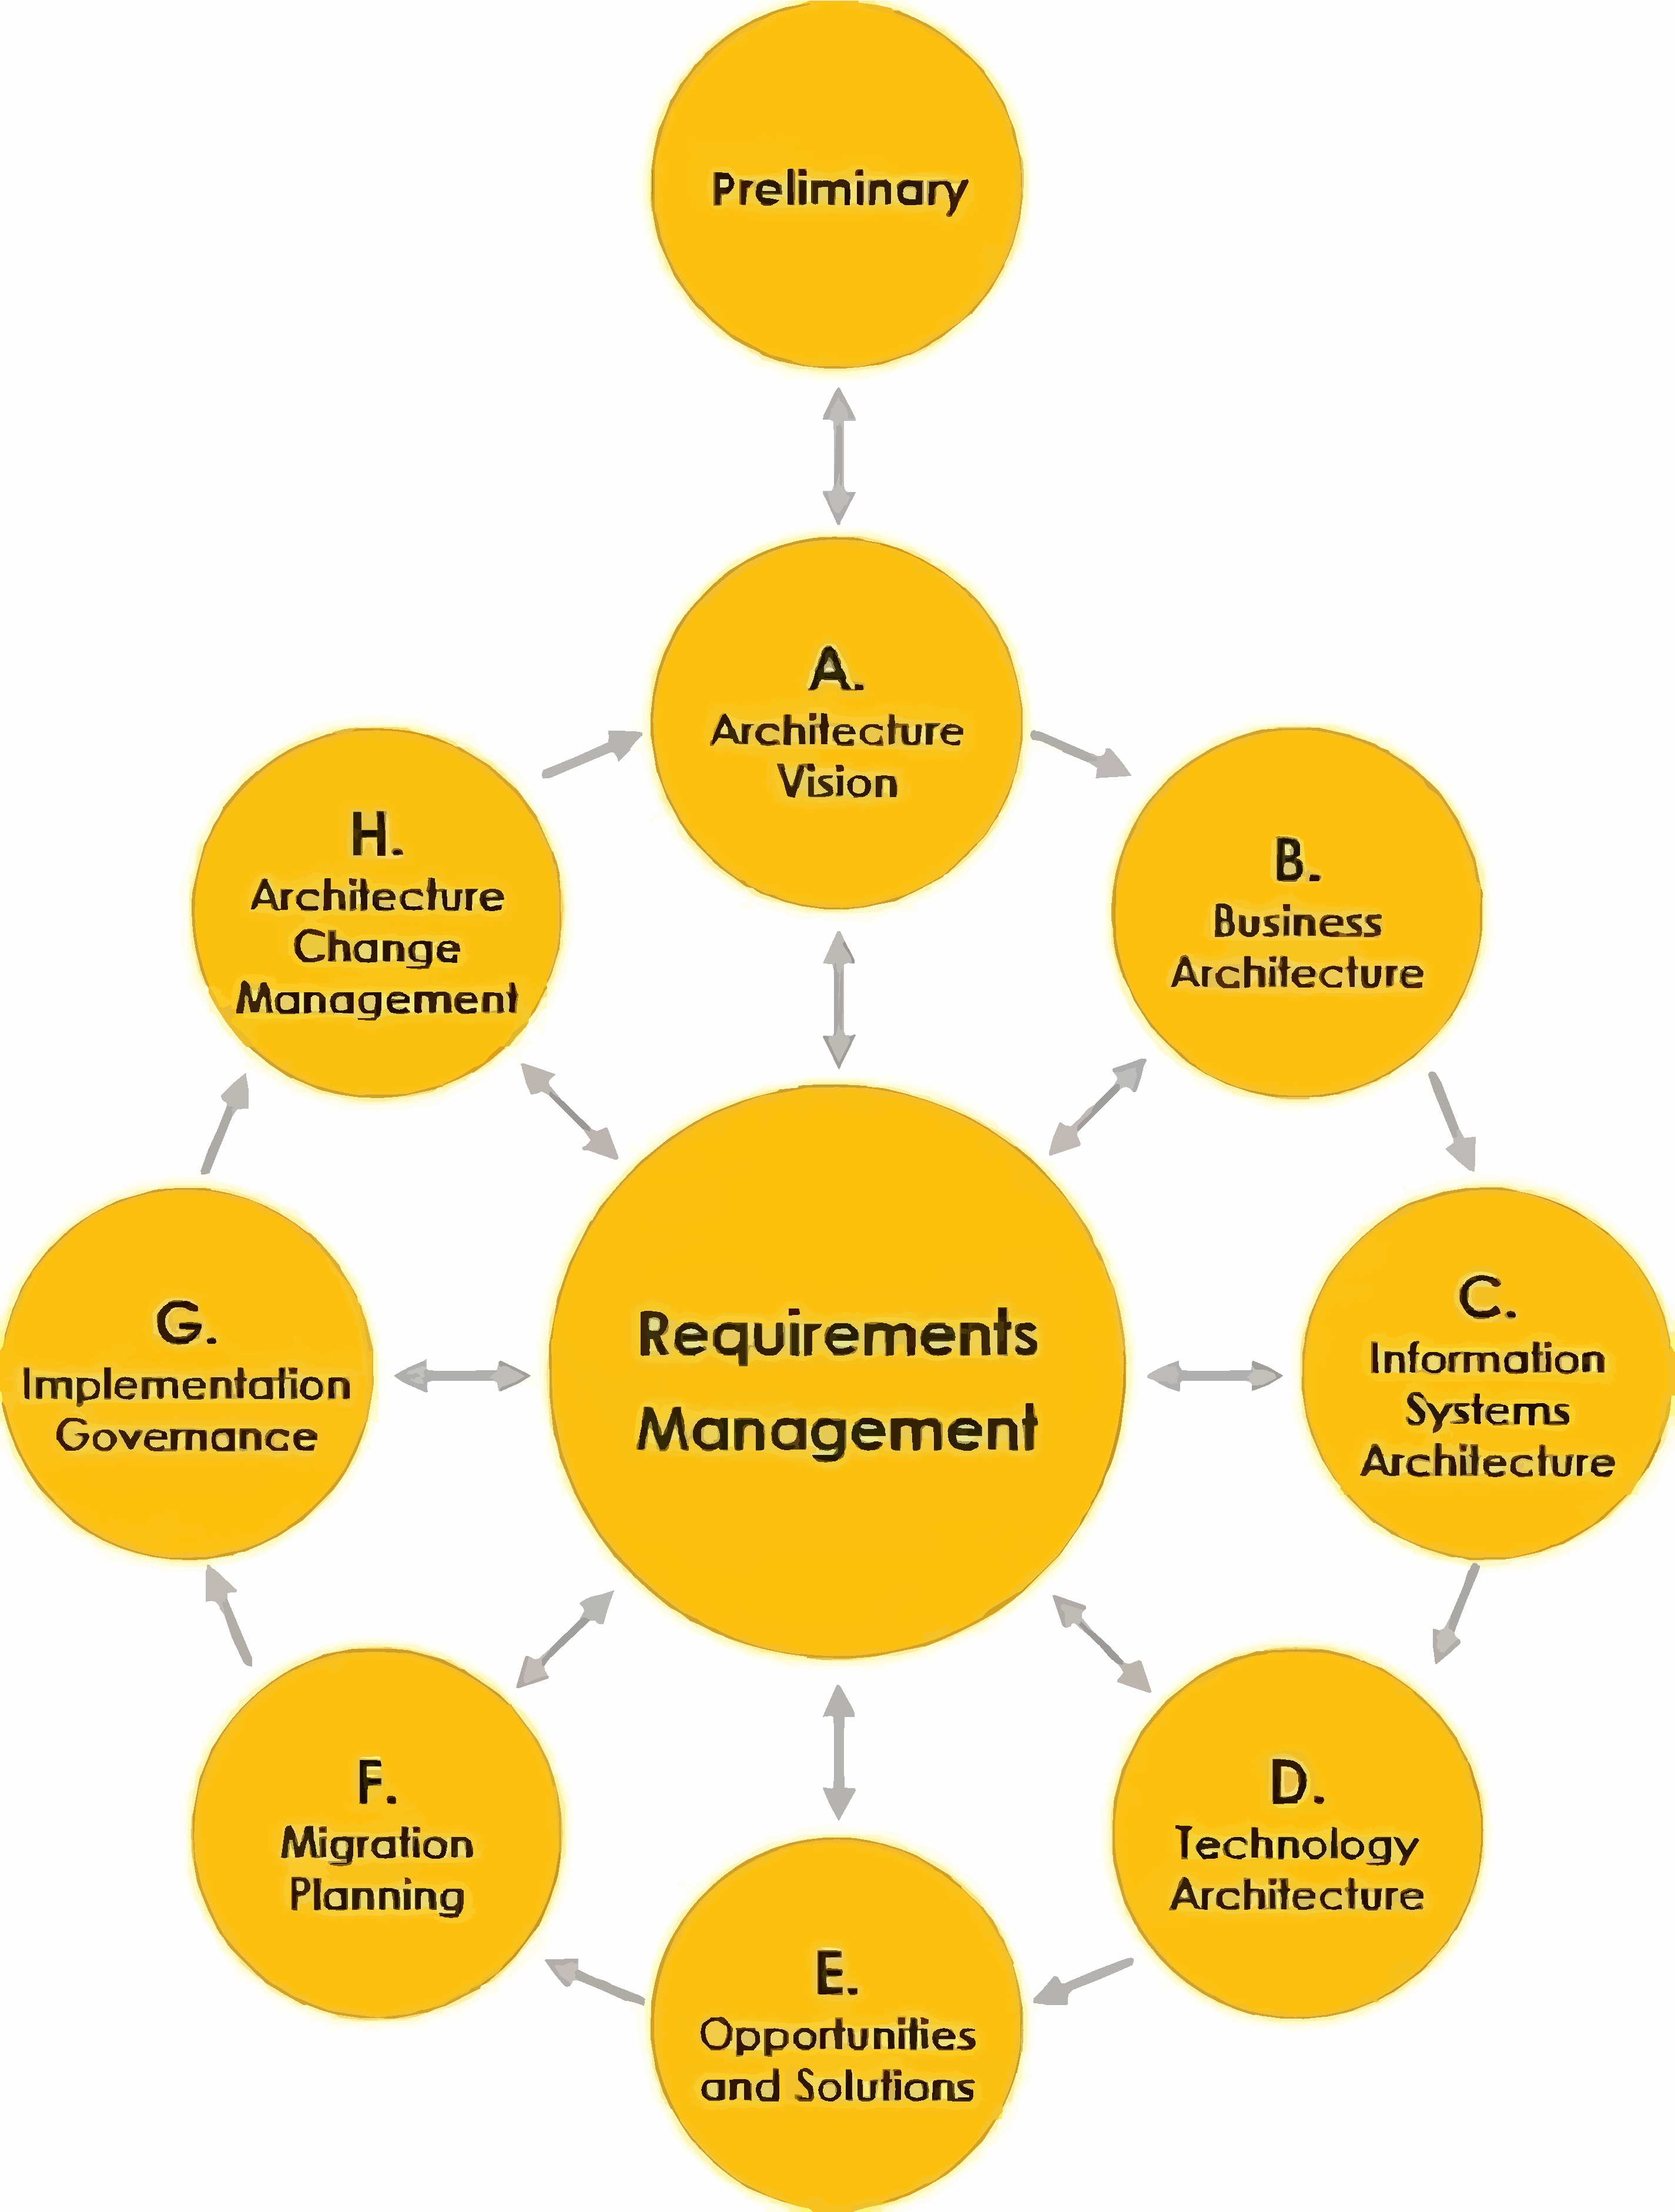
\includegraphics[width=0.7\linewidth]{imgs/Capas ADM.pdf}
	\caption{TOGAF - ADM \cite{capas_ADM}}
	\label{capas-ADM}
\end{figure}

\section{Características de ADM}
El ADM se distingue por ofrecer un enfoque sistemático y adaptable para construir y mantener arquitecturas empresariales robustas. Sus principales características incluyen:

\begin{itemize}
	\item \textbf{Fases y ciclo de vida:} Comprende una secuencia estructurada de fases que abarcan desde la identificación de requerimientos hasta la implementación y gobernanza. Estas etapas conforman un ciclo de vida continuo que permite una evolución coherente de la arquitectura (ver Figura \ref{capas-ADM}).
	
	\item \textbf{Enfoque iterativo:} Las fases se ejecutan de forma iterativa, permitiendo refinar constantemente los modelos y garantizar su alineación con las dinámicas cambiantes del negocio.
	
	\item \textbf{Modularidad y reutilización:} ADM fomenta la creación de artefactos reutilizables y promueve un desarrollo modular que facilita su aplicación en distintos contextos organizacionales.
	
	\item \textbf{Orientación al negocio:} Aunque contempla aspectos técnicos, su enfoque principal es alinear la tecnología con los objetivos estratégicos del negocio, asegurando así una arquitectura que impulse la eficiencia organizacional.
	
	\item \textbf{Apoyo en la toma de decisiones:} Proporciona mecanismos para recopilar, analizar y comunicar información clave que sustente decisiones arquitectónicas informadas.
\end{itemize}

\section{Fases de ADM}
A continuación, se detallan las fases que componen el ciclo de ADM:

\begin{itemize}
	\item \textbf{Preliminar:} Prepara a la organización para emprender iniciativas de arquitectura, adaptando TOGAF a su contexto, seleccionando herramientas y definiendo principios arquitectónicos.
	
	\item \textbf{Gestión de requerimientos:} Asegura que las decisiones arquitectónicas estén alineadas con los requerimientos del negocio, gestionándolos de manera centralizada durante todo el ciclo.
	
	\item \textbf{Fase A - Visión de la arquitectura:} Establece el alcance, objetivos y contexto del proyecto, identificando interesados y definiendo la declaración de trabajo arquitectónica.
	
	\item \textbf{Fase B - Arquitectura de negocio:} Desarrolla la arquitectura empresarial desde una perspectiva funcional, alineada con la estrategia de la organización.
	
	\item \textbf{Fase C - Arquitectura de sistemas de información:} Comprende el desarrollo de la arquitectura de datos y aplicaciones que soportan los procesos del negocio.
	
	\item \textbf{Fase D - Arquitectura tecnológica:} Define la infraestructura tecnológica necesaria para soportar los sistemas y servicios definidos en fases anteriores.
	
	\item \textbf{Fase E - Oportunidades y soluciones:} Identifica proyectos y componentes clave para implementar la arquitectura, considerando alternativas y enfoques de entrega.
	
	\item \textbf{Fase F - Planificación de migración:} Elabora un plan detallado para transitar desde la arquitectura actual hacia la deseada, priorizando iniciativas y recursos.
	
	\item \textbf{Fase G - Gobernanza de implementación:} Supervisa la ejecución técnica para asegurar el cumplimiento con la arquitectura aprobada.
	
	\item \textbf{Fase H - Gestión del cambio:} Evalúa continuamente la arquitectura y propone mejoras conforme evolucionan las necesidades del negocio.
\end{itemize}

Estas fases, al ejecutarse dentro de un ciclo iterativo, permiten a las organizaciones transformar su arquitectura de forma ordenada, maximizando el valor estratégico de sus inversiones tecnológicas.
